%DO NOT MESS AROUND WITH THE CODE ON THIS PAGE UNLESS YOU %REALLY KNOW WHAT YOU ARE DOING
\chapter{Introduction} \label{Introduction}
\section{Preamble} \label{Preamble}
\noindent Internet of Things (IoT) refers to the network of physical objects having the ability to communicate with each other in an ubiquitous way through different technologies. They are used to ensure communication services in many application scenarios such as healthcare, industrial automation, and smart homes. However, sensor nodes are small and battery powered. Thus, changing their batteries is a very challenging task. Low power and Lossy Network (LLN) possess two key features: the limited resources of nodes and the lossy links between them. By considering these specific characteristics, Routing Over Low power and Lossy networks (ROLL) working group has initially proposed the IPv6 standard routing protocol for low power and lossy networks (RPL).\\
\noindent second para\\
\section{Motivation}\label{Motivation}
\noindent This is how you create bullets:\\
\vspace{-1cm}
\begin{itemize}
\item Standard routing protocols like OSPF are inefficient for low power lossy networks (LLNs) due to the constraints and fuzzy nature
\item Using just one metric for the objective function makes the routing protocol unable to accommodate application requirements many a times
\item Some kind of metric combination is required. In this project we use Fuzzy logic to combine ETX, PDR, Hop count and Delay to a metric called Qos(Quality of service).

\end{itemize}
%\section{Objective} \label{Objective}
%\noindent same way
\section{Outline} \label{Outline}
The IPv6 Routing Protocol for Low power and Lossy Networks (RPL) is the standard IPv6 based routing protocol for Low Power, Lossy Networks (LLNs) which consist largely of constrained nodes with limited power, memory, and processing resources like WSNs(Wireless Sensor Networks).RPL uses Objective functions(OFs) to build networks according to these constraints.\\
\noindent\textbf{RPL supports traffic flows like:\\}
\vspace{-1cm}
\begin{itemize}
\item Multipoint-to-poitn - the dominant traffic pattern
\item Point-to-multipoint - using destination advertisement mechanism
\item Point-to-Point
\end{itemize}
\begin{figure}[h!]
\centering
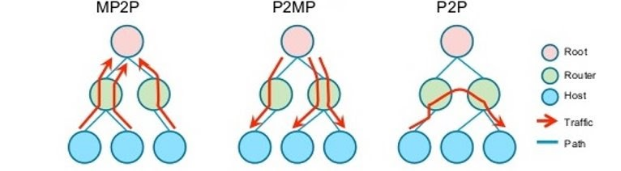
\includegraphics[width=110mm]{traffic flow in rpl.png}
\caption{traffic flow in rpl}
\end{figure}
\subsection{Topology} \label{Topology}
RPL organizes a network topology as a Directed Acyclic Graph (DAG) that is partitioned into one or more Destination Oriented DAGs (DODAGs), one DODAG per sink(root).\\
\begin{figure}[h!]
\centering
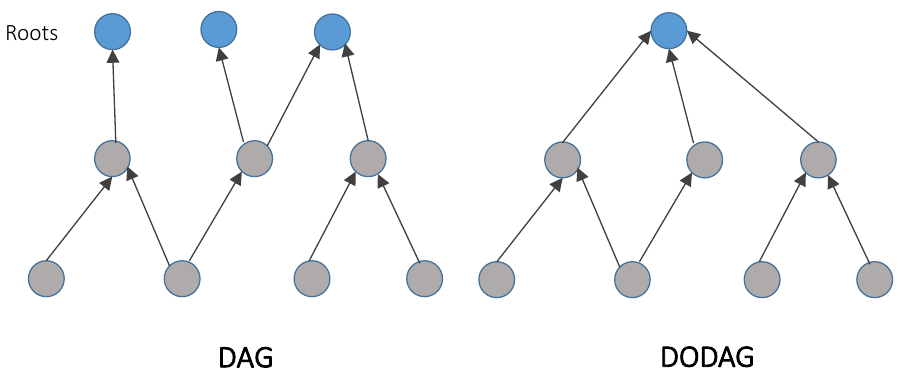
\includegraphics[width=110mm]{dag.png}
\caption{Topology in RPL}
\end{figure}
\begin{itemize}
\item The topology building starts at the root (initially, the only router that is part of the dodag). It sends DIO messages in its neighbourhood(This message contains all common communication parameters, including root ID, modes of operation, timer values etc.)Upon receipt of a number of such messages, neighbour nodes may participate in the DODAG according to the objective function (OF), select their parents and then start emitting their own DIO messages.This process spreads gradually to cover the whole network as new nodes join the DODAG.
\item Prefered Parent- Only one node among parent’s nodes (the preferred parent)acts as the nexthop on the path towards theroot
\item RPL pro-actively creates and maintains the topology, by regularly sending ICMP control messages in the vicinity. The frequency of these exchanges are governed by the Trickle algorithm.
\end{itemize}
\subsection{Important terminology} \label{Important Terminology}
\textbf{RPLInstanceID:}  A RPLInstanceID identifies a set of one or more Destination Oriented DAGs (DODAGs).  A network may have multiple RPLInstanceIDs, each of which defines an independent set of DODAGs, which may be optimized for different Objective Functions (OFs) and/or applications.  The set of DODAGs identified by a RPLInstanceID is called a RPL Instance.  All DODAGs in the same RPL Instance use the same OF.\\
\textbf{Rank:} Rank defines individual node positions with respect to the DODAG root.\\
\textbf{DODAGVersionNumber:} A DODAG version is a specific iteration of a DODAG with a given DODAG ID. DODAGVersionNumber is a sequential counter incremented by the Root to form a new DODAG Version.\\
\textbf{DODAGID:} The combination of RPLInstanceID and DODAGID uniquely identifies a single DODAG in the network.  A RPL Instance may have multiple DODAGs, each of which has an unique DODAGID.\\
\begin{figure}[H]
\centering
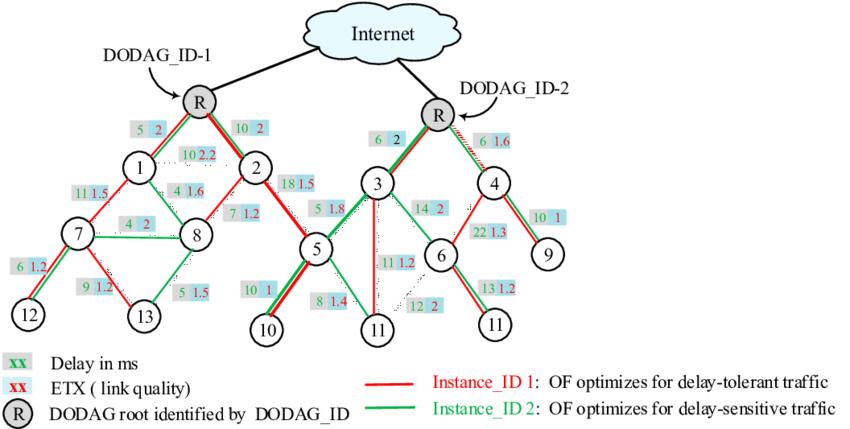
\includegraphics[width=150mm]{dag_structure.png}
\caption{Terminologies used in RPL}
\end{figure}
\subsection{ICMPv6 RPL control message} \label{ICMPv6 RPL Control message}
A RPL control message is identified by a code and composed of a base that depends on the code (and a series of options).\\
In accordance with [RFC4443], the RPL Control Message consists of an ICMPv6 header followed by a message body.  The message body is comprised of a message base and possibly a number of options as illustrated in Figure 1.4.\\
\begin{figure}[H]
\centering
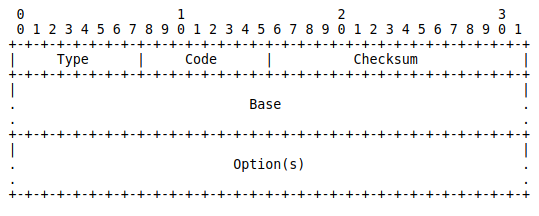
\includegraphics[width=110mm]{RPL control message.png}
\caption{RPL control message}
\end{figure}
\noindent\textbf{DODAG Information Solicitation (DIS)}\\
The DODAG Information Solicitation (DIS) message may be used to solicit a DODAG Information Object from a RPL node.  Its use is analogous to that of a Router Solicitation as specified in IPv6 Neighbor Discovery; a node may use DIS to probe its neighborhood for nearby DODAGs.\\
\noindent\textbf{DODAG Information Object(DIO)}\\
The DODAG Information Object carries information that allows a node to discover a RPL Instance, learn its configuration parameters, select a DODAG parent set, and maintain the DODAG.\\
\noindent\textbf{The Destination Advertisement Object (DAO)}\\
The DAO is used to propagate destination information Upward along the DODAG.  In Storing mode, the DAO message is unicast by the child to the selected parent(s). In Non-Storing mode, the DAO message is unicast to the DODAG root. The DAO message may optionally, upon explicit request or error, be acknowledged by its destination with a Destination Advertisement Acknowledgement (DAO-ACK) message back to the sender of the DAO.\\
\noindent\textbf{DAO Acknowledgement}\\
The DAO-ACK message is sent as a unicast packet by a DAO recipient (a DAO parent or DODAG root) in response to a unicast DAO message.\\

\pagebreak